\documentclass{article}\usepackage[]{graphicx}\usepackage[]{color}
%% maxwidth is the original width if it is less than linewidth
%% otherwise use linewidth (to make sure the graphics do not exceed the margin)
\makeatletter
\def\maxwidth{ %
  \ifdim\Gin@nat@width>\linewidth
    \linewidth
  \else
    \Gin@nat@width
  \fi
}
\makeatother

\definecolor{fgcolor}{rgb}{0.345, 0.345, 0.345}
\newcommand{\hlnum}[1]{\textcolor[rgb]{0.686,0.059,0.569}{#1}}%
\newcommand{\hlstr}[1]{\textcolor[rgb]{0.192,0.494,0.8}{#1}}%
\newcommand{\hlcom}[1]{\textcolor[rgb]{0.678,0.584,0.686}{\textit{#1}}}%
\newcommand{\hlopt}[1]{\textcolor[rgb]{0,0,0}{#1}}%
\newcommand{\hlstd}[1]{\textcolor[rgb]{0.345,0.345,0.345}{#1}}%
\newcommand{\hlkwa}[1]{\textcolor[rgb]{0.161,0.373,0.58}{\textbf{#1}}}%
\newcommand{\hlkwb}[1]{\textcolor[rgb]{0.69,0.353,0.396}{#1}}%
\newcommand{\hlkwc}[1]{\textcolor[rgb]{0.333,0.667,0.333}{#1}}%
\newcommand{\hlkwd}[1]{\textcolor[rgb]{0.737,0.353,0.396}{\textbf{#1}}}%
\let\hlipl\hlkwb

\usepackage{framed}
\makeatletter
\newenvironment{kframe}{%
 \def\at@end@of@kframe{}%
 \ifinner\ifhmode%
  \def\at@end@of@kframe{\end{minipage}}%
  \begin{minipage}{\columnwidth}%
 \fi\fi%
 \def\FrameCommand##1{\hskip\@totalleftmargin \hskip-\fboxsep
 \colorbox{shadecolor}{##1}\hskip-\fboxsep
     % There is no \\@totalrightmargin, so:
     \hskip-\linewidth \hskip-\@totalleftmargin \hskip\columnwidth}%
 \MakeFramed {\advance\hsize-\width
   \@totalleftmargin\z@ \linewidth\hsize
   \@setminipage}}%
 {\par\unskip\endMakeFramed%
 \at@end@of@kframe}
\makeatother

\definecolor{shadecolor}{rgb}{.97, .97, .97}
\definecolor{messagecolor}{rgb}{0, 0, 0}
\definecolor{warningcolor}{rgb}{1, 0, 1}
\definecolor{errorcolor}{rgb}{1, 0, 0}
\newenvironment{knitrout}{}{} % an empty environment to be redefined in TeX

\usepackage{alltt}
\usepackage{Sweave}
\usepackage{float}
\usepackage{graphicx}
\usepackage{tabularx}
\usepackage{siunitx}
\usepackage{amssymb} % for math symbols
\usepackage{amsmath} % for aligning equations
\usepackage{textcomp}
\usepackage{mdframed}
\usepackage{natbib}
\bibliographystyle{..//bib/styles/besjournals.bst}
\usepackage[small]{caption}
\setlength{\captionmargin}{30pt}
\setlength{\abovecaptionskip}{0pt}
\setlength{\belowcaptionskip}{10pt}
\topmargin -1.5cm        
\oddsidemargin -0.04cm   
\evensidemargin -0.04cm
\textwidth 16.59cm
\textheight 21.94cm 
%\pagestyle{empty} %comment if want page numbers
\parskip 7.2pt
\renewcommand{\baselinestretch}{1.5}
\parindent 0pt
%\usepackage{lineno}
%\linenumbers

\newmdenv[
  topline=true,
  bottomline=true,
  skipabove=\topsep,
  skipbelow=\topsep
]{siderules}

%% R Script


\IfFileExists{upquote.sty}{\usepackage{upquote}}{}
\begin{document}
\noindent \textbf{\Large{Regional Risk Outline}}

\noindent Authors:\\
C. J. Chamberlain $^{1,2}$, B. I. Cook $^{3}$, I. Morales Castilla $^{1,4}$ \& E. M. Wolkovich $^{1,2}$
\vspace{2ex}\\
\emph{Author affiliations:}\\
$^{1}$Arnold Arboretum of Harvard University, 1300 Centre Street, Boston, Massachusetts, USA; \\
$^{2}$Organismic \& Evolutionary Biology, Harvard University, 26 Oxford Street, Cambridge, Massachusetts, USA; \\
$^{3}$NASA Goddard Institute for Space Studies, New York, New York, USA; \\
$^{4}$Edificio Ciencias, Campus Universitario 28805 Alcalá de Henares, Madrid, Spain \\
\vspace{2ex}
$^*$Corresponding author: 248.953.0189; cchamberlain@g.harvard.edu\\

\renewcommand{\thetable}{\arabic{table}}
\renewcommand{\thefigure}{\arabic{figure}}
\renewcommand{\labelitemi}{$-$}
\setkeys{Gin}{width=0.8\textwidth}

%%%%%%%%%%%%%%%%%%%%%%%%%%%%%%%%%%%%%%%%%%%%%%%
%%%%%%%%%%%%%%%%%%%%%%%%%%%%%%%%%%%%%%%%%%%%%%%

\section*{Abstract}
Late spring freezing events, also known as false springs, can be ecologically damaging to many plants. A number of studies have found evidence that these events have become more frequent with climate change, but some studies have found the reverse. These diverging results across studies may occur because of the location of studies and because most investigate differing regional and climatic effects linked to false spring risk, which have shifted with climate change. However none have compared multiple factors at once. Using PEP725 leafout data for six tree species across 11,648 sites in Europe, we assessed the effects of NAO, mean spring temperature, elevation and distance from the coast to determine which factors were the strongest predictors of false spring risk and how these predictors shifted with climate change. 
  \begin{enumerate}
    \item Overall, false spring risk decreased with climate change for all species. % however, there was a slight increase in false spring risk with climate change at sites further from the coast. ... EMW: Don't need every result in the abstract, pick the major ones!
        \item Species varied highly in their risk of false springs, however species that initiated budburst early did not always have an increased risk of false spring.
  \item Mean spring temperature and elevation were the strongest predictors of false spring risk, with higher mean spring temperatures having fewer false springs and higher elevations experiencing more false springs. % Is species the strongest overall predictor? If so, you could say here, then move to the climatic predictors. 
  \item Our results suggest that considering multiple regional and climatic factors is essential for predicting false spring risk. % and that these factors better predict false spring risk than budburst date alone. ... EMW: Not sure what you mean here, and not sure it's critical for intro (may be too wordy to explain in intro). 
%   \item More robust observational data that include both budburst and leafout times are crucial for forecasting false spring risk more accurately. %EMW: I  would include this in the discussion, but not here.  If you want another closing sentence you could focus on next steps more strongly linked to your findings, but I think this abstract as is is a great start. 
  \end{enumerate}

\section*{Introduction}
Temperate tree and shrub species are at risk of damage from late spring freezing events, also known as false springs, and this risk may shift with climate change. The growing season is lengthening (mainly due to earlier springs) across many regions in the northern hemisphere \citep{Chen2005, Liu2006, Kukal2018}, but last spring frosts still pose a threat in many of these regions \citep{Wypych2016a}. Spring onset is advancing, with temperate tree and shrub species initiating leafout 4-6 days on average earlier per $^{\circ}$C of warming \citep{Wolkovich2012, IPCC2014}. Last spring freeze dates are not predicted to advance at the same rate \citep{Inouye2008, Martin2010, Labe2016, Sgubin2018}, potentially amplifying the effects of false spring events in these regions. In Germany, for example, the last freeze date has advanced by 2.6 days per decade since 1955 \citep{Zohner2016} but budburst is advancing around twice as fast. Major false spring events have been recorded in recent years and have found it can take 16-38 days for trees to refoliate \citep{Gu2008, Augspurger2009, Augspurger2013, Menzel2015}, which can detrimentally affect crucial processes such as carbon updake and nutrient cycling \citep{Hufkens2012, Richardson2013, Klosterman2018}.

Episodic frosts are one of the largest limiting factors in species range limits and have shaped plant life history strategies \citep{Kollas2014}. Temperate plants are exposed to freezing temperatures numerous times throughout the year, however, individuals are most at risk to damage from spring frosts, when frost tolerance is lowest \citep{Sakai1987}. Plants can avoid damage by carefully timing budburst each year. Indeed, trees and shrubs in temperate regions optimize growth and minimize frost risk by using a complex mix of cues to initiate budburst: low winter temperatures, warm spring temperatures, and increasing spring daylengths. With climate change advancing, this interaction of cues may shift spring phenologies both across and within species, making some species less -- or more --- vulnerable to false springs than before. Early-leafout species may be especially at risk.
 
Plants are least frost resistant during certain phenophases. Frost tolerance greatly diminishes once individuals exit the dormancy phase (i.e. processes leading to budburst) through full leaf expansion \citep{Vitasse2014, Lenz2016}. Individuals that initiate budburst and have not fully leafed out before the last spring freeze are at risk of leaf tissue loss, damage to the xylem, and slowed canopy development \citep{Gu2008, Hufkens2012}. Thus, It is important to consider the length of time between budburst and leafout --- when individuals are most at risk to spring freeze damage \citep{Lenz2016} --- in order to better predict false spring risk. We will refer to this timing between budburst and leafout as the duration of vegetative risk (Rethinking).

Given its importance to plant performance and survival, understanding how false spring is shifting with climate change has been a major topic in the literature. There is large debate over whether or not spring freeze damage will increase \citep{Hannenin1991, Augspurger2013, Labe2016}, remain the same \citep{Scheifinger2003} or even decrease \citep{Kramer1994, Vitra2017} with climate change and there is also great variation within studies. Some research suggests false spring incidence has already begun to decline in many regions (i.e. across parts of North America and Asia), however the prevalence of spring frosts has consistently increased across Europe since 1982 \citep{Liu2018}. Furthermore, recent studies have demonstrated site effects may be more closely related to false spring risk: whether via altitudinal variation \citep{Vitra2017, Ma2018} or distance from the coast \citep{Wypych2016a, Ma2018}. By better understanding these regional climatic implications and which factors are most crucial for predicting risk, we may be able to determine which regions may be at risk currently and which regions may become more at risk in the future.

The majority of false spring studies assess the effects of one predictor (e.g. temperature, elevation or distance from the coast) on false spring prevalence but most fail to incorporate multiple effects. Our primary aim is to investigate the known regional factors on false spring risk and compare the effect of them and their interaction with climate change. The key regional factors we identify for this study are: mean spring temperature, elevation and distance from the coast. Given our focus on Europe, we additionally examine the North Atlantic Oscillation (NAO) index, which is tied to winter and spring circulation across Europe. More positive NAO phases tend to result in higher than average winter and spring temperatures. With climate-change induced shifts, higher NAO phases has correlated to even earlier budburst dates since the late 1980s in some regions \citep{Chmielewski2001}, however it is unclear if more positive NAO phases also translates to more false springs.

By refining and identifying budburst and climate trends in recent years, we could improve future projections in false springs. For this purpose, we assessed the number of false springs that occured across 11,648 sites around Europe, spanning altitudinal and coastal gradients, using observed phenological data (754,786 observations) for six temperate, deciduous trees and combined that with daily gridded climate data for each site that extended from 1951-2016. In this study, a false spring was tallied when temperatures fell below -2.2$^{\circ}$ \citep{Schwartz1993} between budburst and leafout (CITE Rethinking here?). Since the primary aim of the study is to predict false spring incidence in a changing climate, we split our data to before and after 1983 to capture reported temporal shifts in temperature trends \citep{Stocker2013, Kharouba2018}. We predicted that: (1) Earlier budburst species would experience more false springs, especially after 1983, (2) there would be different regional effects (i.e. mean spring temperature, NAO index, elevation, distance from the coast) on false spring incidence and those trends would shift when coupled with the effects of climate change 


\section*{Methods}
\subsection*{Phenological Data and Calculating Vegetative Risk}
We obtained phenological data from the Pan European Phenology network (PEP725, www.pep725.edu), which provides open access phenology records across Europe \citep{Templ2018}. Since plants are most susceptible to damage from frost between budburst and full leafout, we selected only leafout data \citep[i.e., in][BBCH 11, which is defined as the point of leaf unfolding and the first visible leaf stalk]{Meier2001} from the PEP725 dataset. The species used in the study were \textit{Aesculus hippocastanum} Poir., \textit{Alnus glutinosa} (L.) Gaertn., \textit{Betula pendula} Roth., \textit{Fagus sylvatica} Ehrh., \textit{Fraxinus excelsior} L., \textit{Quercus robur} L. Selection criteria for the species were as follows: (1) to be temperate, deciduous species that were not cultivars or used for crops, (2) there were at least 90,000 observations of BBCH 11 (leafout), (3) to represent over half of the total number of sites available (11,684), and (4) there were observations for at least 65 out of the 66 years of the study (1951-2016) (Table S1). We then subtracted 12 days from the leafout date to establish a standardized estimate for day of budburst \citep{Donnelly2017}.

\subsection*{Climate Data}
We collected daily gridded climate data from the European Climate Assessment \& Dataset (ECA\&D) and used the E-OBS 0.25 degree regular latitude-longitude grid from version 16. We used the daily minimum temperature dataset to determine if a false spring occurred. False springs in this study were defined as temperatures at or below -2.2$^{\circ}$C \citep{Schwartz1993} during the duration of vegetative risk. In order to capture regional climatic effects we calculated the mean spring temperature by using the daily mean temperature from March 1 through May 31. Mean spring temperature was calculated -- likely after chilling was accummulated -- in an attempt to incorporate the general effects of spring forcing temperatures in our Bayesian hierarchichal model and to compare differences in spring across sites \citep{Basler2012, Korner2016}. We collected NAO-index data from the KNMI Climate Explorer CPC daily NAO time series and selected the NAO indices from November until April to best capture the effects of NAO on budburst for each region and then took the mean NAO indice during these months \citep{NAOdata}. Since the primary aim of the study is to predict false spring incidence in a changing climate, we split the data: before temperature trends increased (1951-1983) and after trends increased \citep[1984-2016,][]{Stocker2013, Kharouba2018} to represent climate change.

\subsection*{Data Analysis}
A false spring was determined if temperatures fell below -2.2$^{\circ}$C at least once between budburst and leafout. We scaled all of the predictors and used a z-score following the binary predictor approach in order to best compare the effects of each climate variable to each other \citep{Gelman2006}. We used a space parameter, rather than a more traditional latitude parameter, to adjust for spatial autocorrelation issues using a minimization of Moran's \textit{I} of the residuals \citep{Baumen2017} (Figure S1). We then took the calculated eigenvectors determined from the MIR approach and regressed these against the number of false springs for each datapoint to establish a spatial parameter (space). % get citation from Nacho regarding regression

We used a Bayesian hierarchical model approach to analyze our data to best estimate the number of false springs across-species levels. We fit a bernoulli distribution model using mean spring temperature, NAO, elevation, distance from the coast, space, and climate change as predictors and all two-way interactions (fixed effects) and species as two-way interactions to simulate modeled groups on the main effects. The Bayesian hierarchical model was fit using the brms package \citep{brms}, version 2.3.1,  in R \citep{R}, version 3.3.1, and was written as follows: 
\begin{align*} \label{eq:1} 
y_i \thicksim N(\alpha_(i)) +&  \beta_{NAO_{(i)}} + \beta_{MeanSpringTemp_{(i)}} + \beta_{Elevation_{(i)}} + \beta_{DistanceCoast_{(i)}} + \beta_{Space_{(i)}} \\ +& \beta_{ClimateChange_{(i)}}
+ \beta_{NAO \times Species_{(i)}} + \beta_{MeanSpringTemp \times Species_{(i)}} + \beta_{Elevation \times Species_{(i)}} \\ +& \beta_{DistanceCoast \times Species_{(i)}} + \beta_{Space \times Species_{(i)}} + \beta_{ClimateChange \times Species_{(i)}} \\
+& \beta_{NAO \times ClimateChange_{(i)}} + \beta_{MeanSpringTemp \times ClimateChange_{(i)}} 
+ \beta_{Elevation \times ClimateChange_{(i)}} \\ +& \beta_{DistanceCoast \times ClimateChange_{(i)}} + \beta_{Space \times ClimateChange_{(i)}} + \sigma_{sp_{(i)}} 
\end{align*}
%\item The $\beta$ coefficients and $\alpha$ were modeled at the species level:
%\begin{align*}
%1.& \; \beta_{MeanSpringTemp_{sp}} \thicksim N(\mu_{MeanSpringTemp}, \sigma{^2}_{MeanSpringTemp}) \\
%   &... \\
%5.& \; \beta_{ClimateChange_{sp}} \thicksim N(\mu_{ClimateChange}, \sigma{^2}_{ClimateChange})
%\end{align*}
We ran two chains, each with 2,500 warm-up iterations and 4,000 sampling iterations for a total of 8,000 posterior samples for each predictor. We evaluated our model performance on $\hat{R}$ values that were close to one and assessed chain convergence and posterior predictive checks \citep{Gelman2006}.

\subsection*{Testing the rate of budburst on false spring incidence}
The definition of a false spring has been established to be freezing temperatures of -2.2$^{\circ}$C \citep{Schwartz1993} after budburst but plants are most susceptible to damage during the duration of vegetative risk \citep{Augspurger2013, Lenz2016}. Different species have different durations of vegetative risk, which is also shifting with climate change \citep{Cleland2006, Fu2015, Xin2016}. We tested our original model by making a different more biologically relevant model with different durations of vegetative risk for each species. Due to insufficient budburst data from PEP725, we calculated budburst by subtracting 11 days from leafout for \textit{Aesculus hippocastanum} and \textit{Betula pendula}, 12 days for \textit{Alnus glutinosa}, 5 days for \textit{Fagus sylvatica}, and 7 days for \textit{Fraxinus excelsior} and \textit{Quercus robur} based on growth chamber experiment data from phylogenetically related species \citep{Buerki2010, Wang2016, Hipp2017, Flynn2018}.

\section*{Results}
\subsection*{Species variation in budburst and false spring incidence}
\begin{enumerate}
\item There was variation in day of budburst across the six species and across space (Figure \ref{fig:bbmap}). 
\begin{enumerate}
\item The top three species (\textit{Betula pendula}, \textit{Aesculus hippocastanum}), \textit{Alnus glutinosa} generally initiated budburst earlier than the bottom three species (\textit{Fagus sylvatica}, \textit{Quercus robur}, \textit{Fraxinus excelsior}).
%\item Across all species, certain regions tended to initiate budburst earlier than others (i.e. United Kingdom was earlier than parts of Austria).
\end{enumerate}

\item After 1983, all species initiated budburst earlier (Figure \ref{fig:boxfs}A) and the minimum temperature between budburst and leafout was, on average, higher. 
\begin{enumerate}
\item Species that initiated budburst early did not always correspond to a higher risk of false springs (Figure \ref{fig:boxfs}C), as is evident by \textit{Alnus glutinosa}.
\item As seen in Figure \ref{fig:mst}, mean spring temperature for most species ranged from -5$^{\circ}$C to 12$^{\circ}$C, but for \textit{Alnus glutinosa} and \textit{Fraxinus excelsior} the mean spring temperature rarely dropped below 0$^{\circ}$C, whereas \textit{Quercus robur} experienced some of the lowest spring temperatures.
\item The average minimum temperature between budburst and leafout, however, varied across the six species with \textit{Betula pendula} and \textit{Aesculus hippocastanum} experiencing the lowest minimum temperatures (Figure \ref{fig:boxfs}B). 
\end{enumerate}
\end{enumerate}

\subsection*{The effects of climatic regional variation on false spring incidence}
\begin{enumerate}
\item The effects of the predictors varied in both direction and magnitude (Figure \ref{fig:maineffects}).
  \begin{enumerate}
  \item Mean spring temperature had the biggest effect (-1.14) on the number of false springs, with warmer spring temperatures resulting is fewer false springs. 
  \item More positive NAO indices slightly lowered the risk of false spring (-0.11) but higher elevations and sites further from the coast increased the likelihood of false spring incidence: +1.02 and +0.35 respectively.
  \item Overall, there were fewer false springs after 1983. 
  \end{enumerate}
\item Most of the interactions with increasing temperatures (i.e. the Climate Change predictor) exhibit a decreased risk in false springs (from -0.29 to -1.20), however, the probability of false spring incidence increased at sites further from the coast after 1983 (+0.11) (Figure \ref{fig:maineffects}). 
  \begin{enumerate}
  \item After climate change, the rate of false spring incidence decreased with increasing NAO indices (Figure \ref{fig:intrxns}A).
  \item The probability of a false spring was lower at higher elevations after 1983 than before 1983 (Figure \ref{fig:intrxns}B).
  \item After climate change, the probability of a false spring was slightly higher at lower mean spring temperature sites but the probability is slightly lower at higer mean spring temperature sites (Figure \ref{fig:intrxns}C).
  \item There was an increased risk of a false springs further from the coast before and after climate change (Figure \ref{fig:intrxns}D).
  \end{enumerate}
\item The probability of a false spring occurring varied by species with each predictor (Figure \ref{fig:spp}).
  \begin{enumerate}
  \item With increasing mean spring temperatures, there were fewer false springs for each species, however \textit{Aesculus hippocastanum} had the greatest risk of false springs and \textit{Fraxinus excelsior} had the lowest risk. 
  \item With increasing elevation, \textit{Betula pendula} had the greatest risk of a false spring occurring and the risk also increased for \textit{Aesculus hippocastanum} and \textit{Quercus robur}. 
  \item All other predictors did not drastically affect the probability of false spring risk at the species level.
\end{enumerate}
\end{enumerate}

\subsection*{Standardized rate of budburst}
%\item By changing the temperature threshold for defining a false spring --- from -2.2$^{\circ}$C to -5$^{\circ}$C --- many of the predictors changed in both magnitude and direction but overall there were fewer false springs (Figure \ref{fig:five}).
\begin{enumerate}
%\item With a lower false spring temperature, increasing elevation greatly increased the risk of a false spring and more positive NAO indices after climate change also increased the risk of false springs.
%\end{enumerate}

\item By having different durations of vegetative risk for each species the magnitude and direction of the predictors remained consistent with the original model (Figure S2). %\ref{fig:orig})
  \begin{enumerate}
  \item There were fewer false springs after 1983 and mean spring temperature and elevation were the strongest predictors for false spring risk. 
  \item And, again, distance was the only, albeit weakly, positive interaction effect with climate change. 
  \end{enumerate}

\end{enumerate}  
  
  
%\item Standardizing the rate of budburst to 12 days between budburst and leafout across all species also changed the magnitude and direction of some predictors (Figure). %\ref{fig:orig})
 % \begin{enumerate}
  %\item More positive NAO indices resulted in a slightly decreased risk of false springs. 
  %\item Higher elevations greatly increased the risk of a false spring.
%\end{enumerate}
%\end{enumerate}


\section*{Discussion}
\begin{enumerate}
\item There is robust evidence for advancing budburst with climate change \citep{Cleland2007, Wolkovich2012, IPCC2014} and some studies indicate earlier budburst species are more at risk of false spring damage \citep{Ma2018}.
  \begin{enumerate}
  \item After 1983, all of our species initiated budburst earlier in the spring but there was a decrease overall in false spring risk.
  \item Additionally, some of the early bursting species were more susceptible to false spring risk (i.e. \textit{Betula pendula} and \textit{Aesuculus hippocastanum}) but not all early bursting species were at a higher risk of false springs (i.e. \textit{Alnus glutinosa}). 
  \item Thus, simply looking at budburst time is not a sufficient proxy to forecast false spring risk and other climatic and regional factors must be evaluated.
  \end{enumerate}
  
\item Past studies using single predictors for false spring events has lead to contradicting predictions in future false spring risk.
  \begin{enumerate}
  \item Through our holistic approach, we were able to assess the myriad of climatic and regional effects on false spring risk -- and how the magnitude of those effects compare to one another -- by incorporating the space parameter, thus erasing the collinearity issues of certain effects (i.e. elevation and distance from the coast).
  \item This was an essential step in forecasting false spring risk.
  \item Our study supports findings from previous studies: higher elevations tend to experience more false springs but that risk is diminishing with climate change \citep{Vitra2017} and sites that are generally warmer have lower risks of false springs and that risk is decreasing with climate change \citep{Wypych2016}.
  \item However, we also discovered that effects of elevation and distance from the coast cannot be assumed to be the same, which contradicts previous studies \citep{Ma2018}.
  \item Our results suggest that sites further from the coast were the only sites to have a slightly increased risk of false springs with shifts in climate even though sites at higher elevations had a decreased risk over time. 
  \end{enumerate}
  
\item Overall, mean spring temperature and elevation are the best predictors for false spring risk: sites that are warmer generally have fewer false springs and sites that are at higher elevations generally have more false springs.
  \begin{enumerate}
  \item Across our study sites, budburst initiated earlier after 1983 due to warming temperatures but the minimum temperatures also increased, suggesting false spring risk is diminishing over time. 
  \item Our results also indicate that higher NAO indices --- which typically leads to earlier budburst --- also reduced the risk of false springs and that risk diminished further over time.
  \end{enumerate}
\item However, our study fails to assess the intensity or severity of the false spring events. 
  \begin{enumerate}
  \item It is possible that even though the frequency, or probability, of risk is decreasing, false spring events after 1983 could be lasting longer or could at be at even harsher temperatures.
  \item Additionally, there is sufficient evidence that different species are able to tolerate different minimum temperature extremes \citep{Lenz2013, Korner2016, Zhuo2018}.
  \item Some species or individuals may be less tolerant of low temperatures (i.e. are damaged from higher temperatures than -2.2$^{\circ}$C), whereas other species or individuals may be able to tolerate temperatures as low as -8.5$^{\circ}$C \citep{Lenz2016}.
  \item Thus, species that are typically found in low risk sites but have early budburst (i.e. \textit{Alnus glutinosa}) may be less tolerant of low temperatures and they may be at sites that are further from the coast, which are experiencing a slightly increased risk with climate change. 
  \item For this reason, models should incorporate species-specific temperature thresholds to best capture the shifts in false spring risk over time and space. 
  \end{enumerate}

\item Biological spring is advancing with climate change-induced shifts but few studies have assessed the effects of climate change on the duration of vegetative risk: is leafout advancing at the same rate or is the duration of vegetative risk lengthening?
  \begin{enumerate}
  \item For false spring studies, it is important to consider the effects of climate change on both budburst and leafout, the timing when individuals are most at risk to spring freeze damage \citep{Lenz2016}.
  \item With less chilling, shorter photoperiods but warmer spring temperatures, the duration of vegetative risk could change, thus altering the predicted outcome of false spring risk.
  \item And with changing rates of budburst, the regional and climatic effects will impact the number of false springs an individual experiences differently.
  \item Incorporating observed durations of vegetative risk across sites, years and species would greatly enhance model predictions. 
  \end{enumerate}
\end{enumerate}
  
\section*{Conclusion}
\begin{enumerate}
\item False spring risk is influenced by numerous climatic and regional factors and all of these factors must be incorporated into models to best predict spatiotemporal shifts in false springs.
  \begin{enumerate}
  \item Some factors are better at predicting risk than others (i.e. mean spring temperature and elevation), however it is essential to additioanlly assess the effects of NAO and distance from the coast, which also contribute to an individual's risk of false spring. 
  \item Individuals that initiate budburst earlier in the season aren't necessarily exposed to more false springs, thus, investigating site effects is a more consistent proxy for false spring risk than budburst time. 
  \item Overall, the frequency of false spring events is decreasing with climate change but additional studies are crucial to understand how the intensity and duration of these events are shifting.
  \item Furthermore, incorporating both budburst and leafout data as well as species-specific temperature thresholds will advance our knowledge of false spring risk in a changing climate. 
  \end{enumerate}
\end{enumerate}
  
  
  
  
  
  

%
%\end{enumerate}
%\item Individuals from more Northern provenances tend to be more susceptible to spring frost damage, whereas more Southern individuals are more sensitive to fall frosts \citep{Montwe2018}.
%\begin{enumerate}
%\item With regional shifts in climate, will fall frosts become more damaging than spring frosts?
%\end{enumerate}
%\end{enumerate}


\bibliography{..//bib/regionalrisk.bib}

\section*{Tables and Figures} 

{\begin{figure} [H]
  -\begin{center}
  -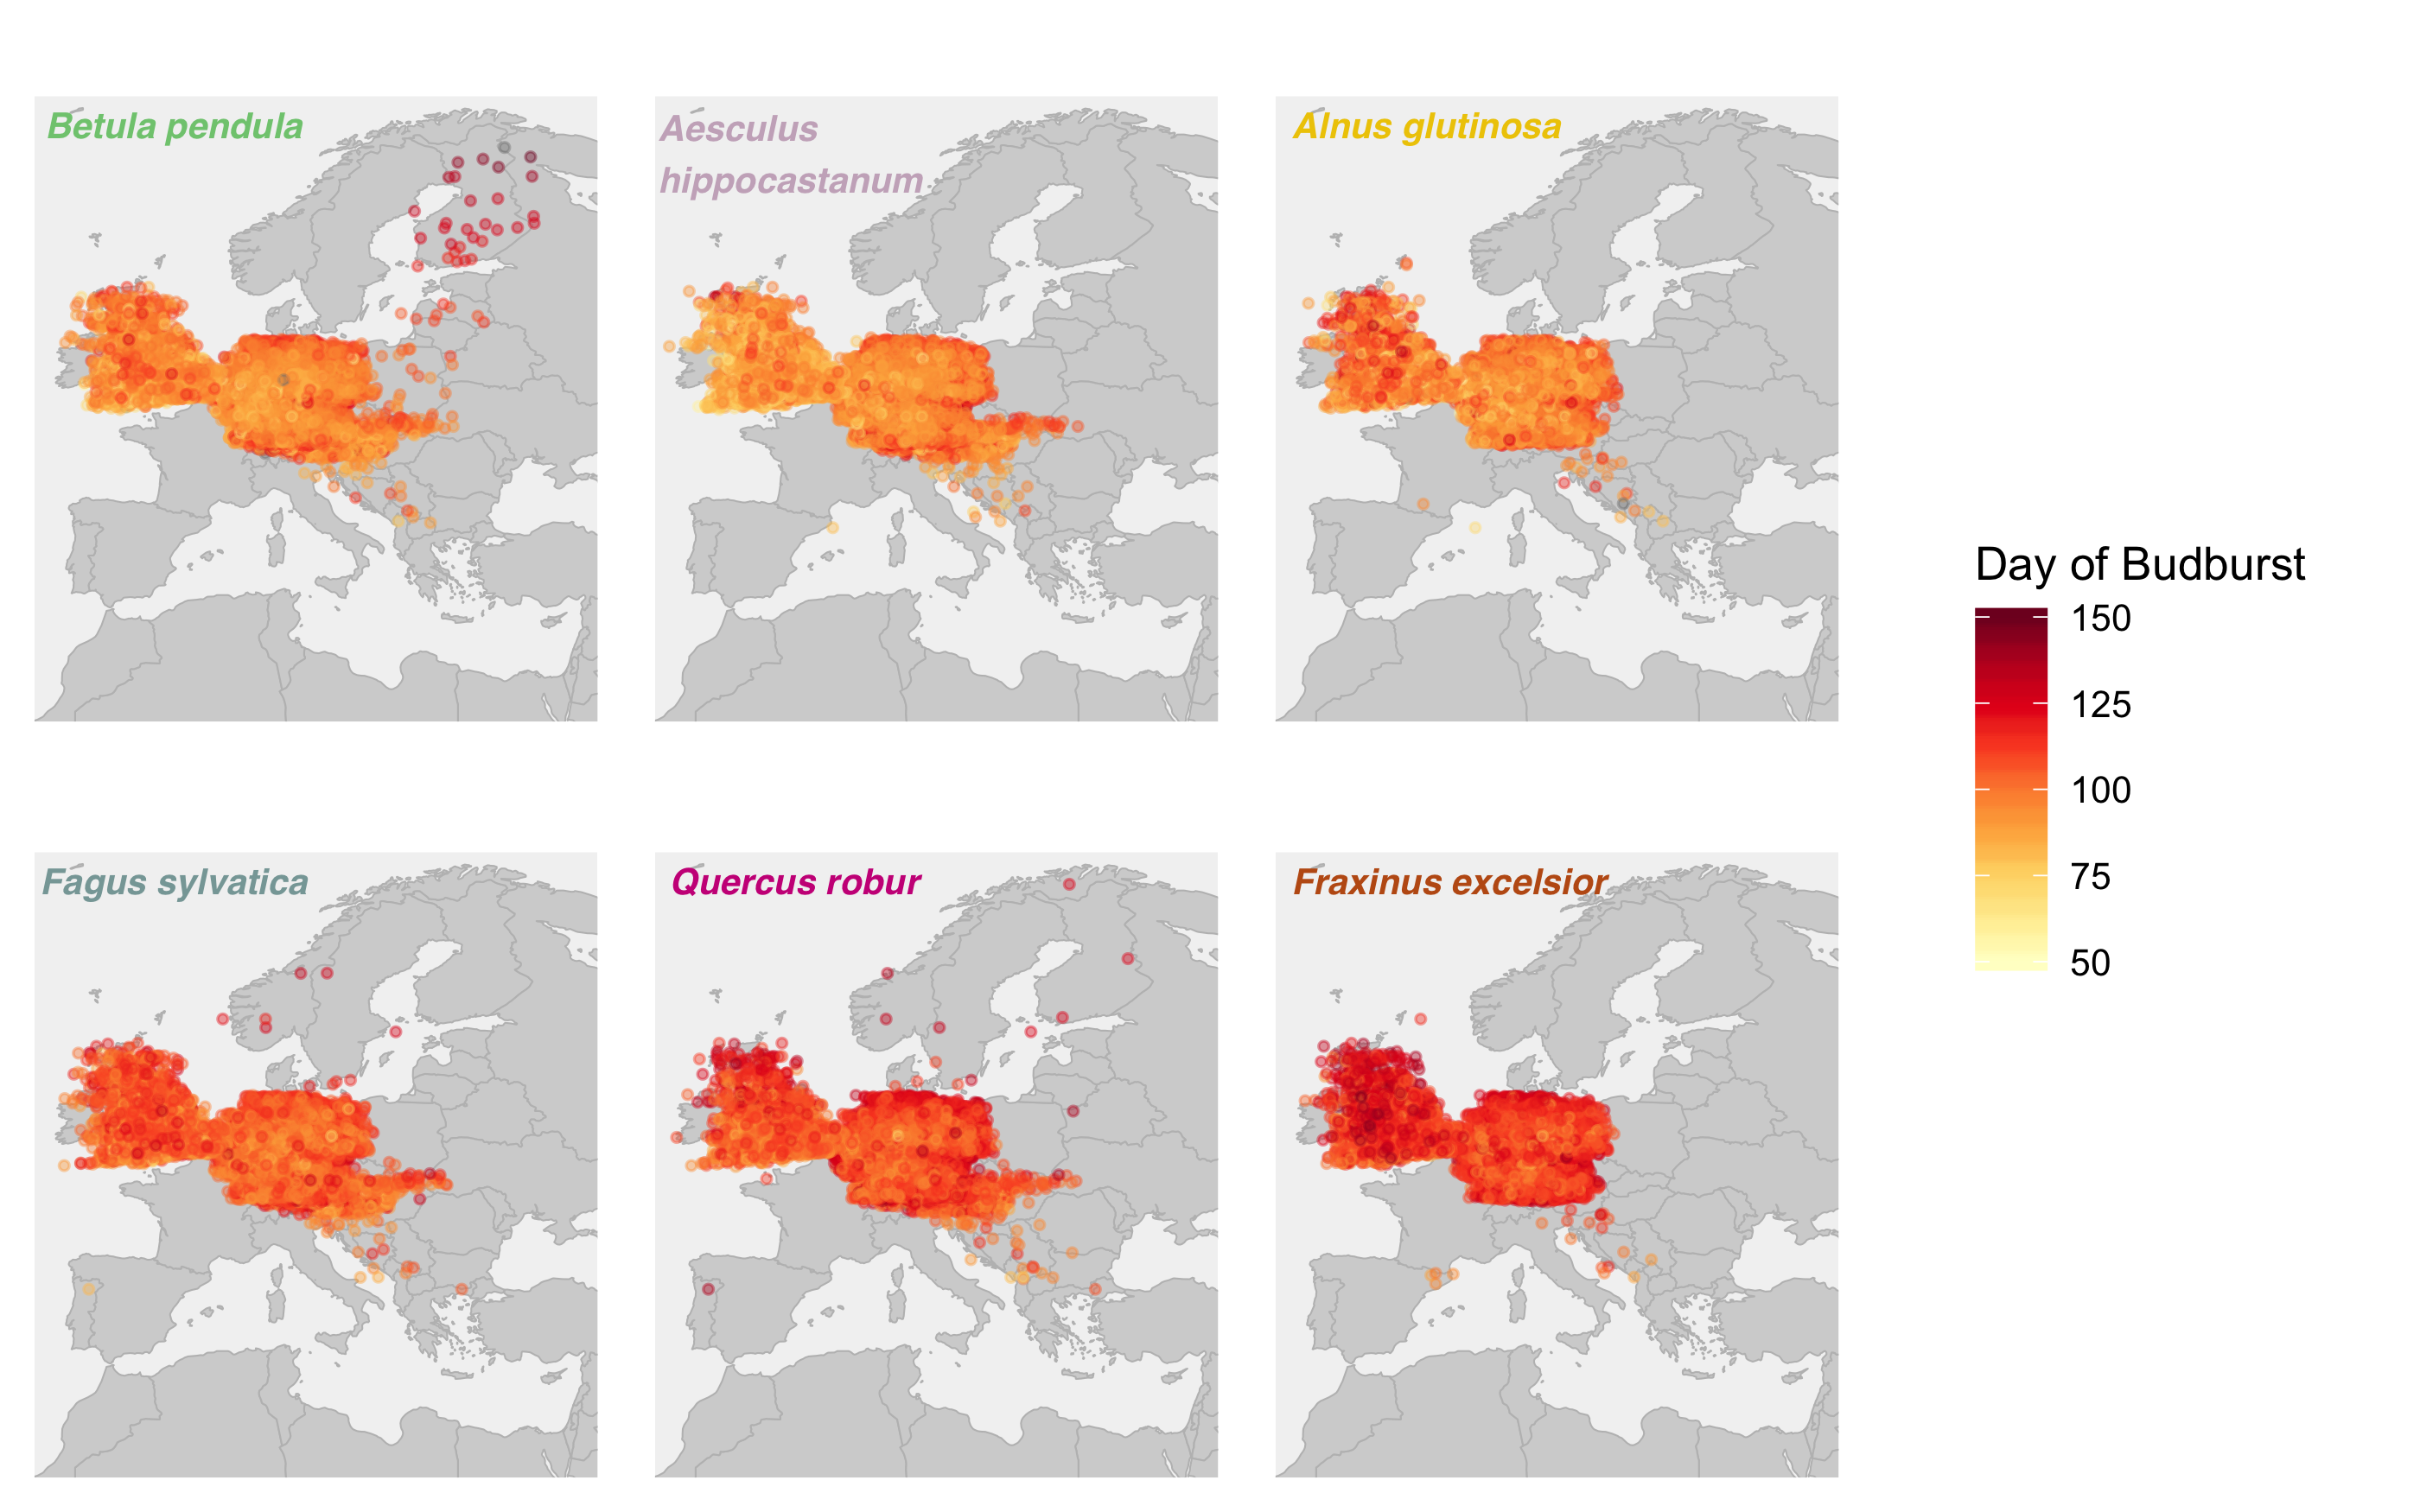
\includegraphics[width=14cm]{..//figures/BB_base.png}
  -\caption{The average day of budburst is mapped by site for each species. Species are ordered by day of budburst starting with \textit{Betula pendula} as the earliest budburst date to \textit{Fraxinus excelsior}. Earlier budburst dates are blue and later budburst dates are in red. }\label{fig:bbmap}
  -\end{center}
  -\end{figure}}
  
{\begin{figure} [H]
  -\begin{center}
  -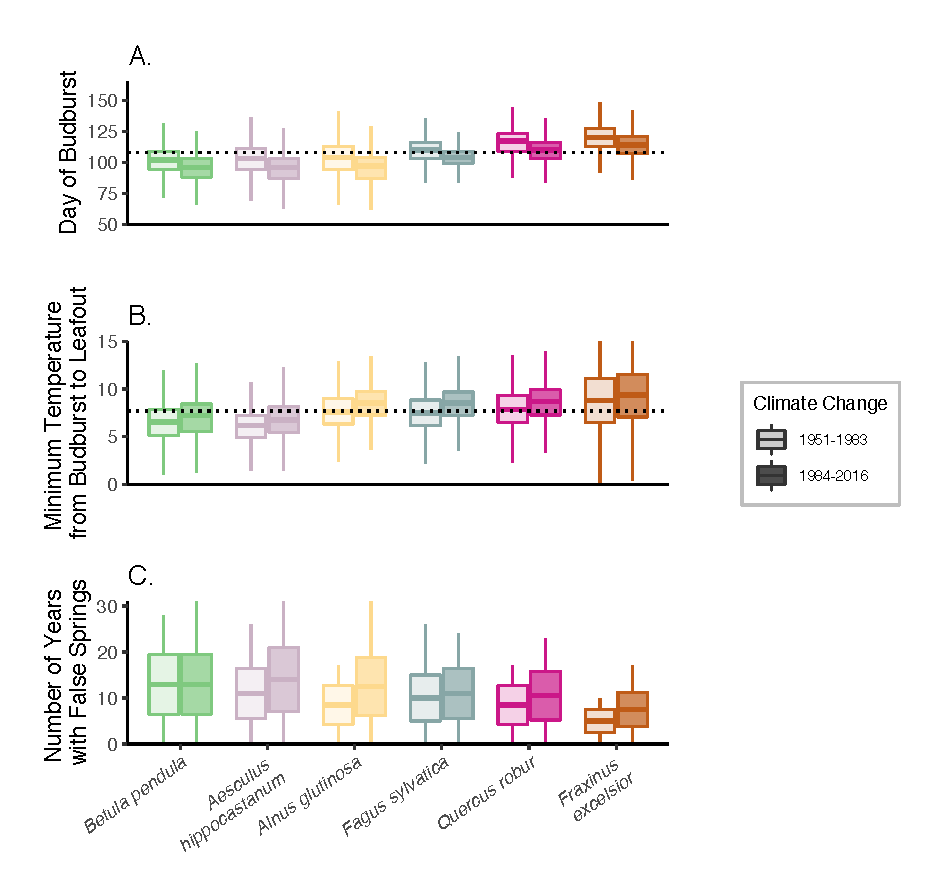
\includegraphics[width=14cm]{..//figures/Boxplot_BBTminFS_noDots.pdf}
  -\caption{Budburst, minimum temperatures and false springs were compared before and after 1983 for each species. We plotted the day of budburst (A.) before and after 1983 for each species across all sites. We then compared the average minimum temperatures (B.) between budburst and leafout for all species across all sites. The bottom panel (C.), shows the total number of years there was a false spring before and after 1983 at each site across all species. Species are ordered by day of budburst.  }\label{fig:boxfs}
  -\end{center}
  -\end{figure}}
  
{\begin{figure} [H]
  -\begin{center}
  -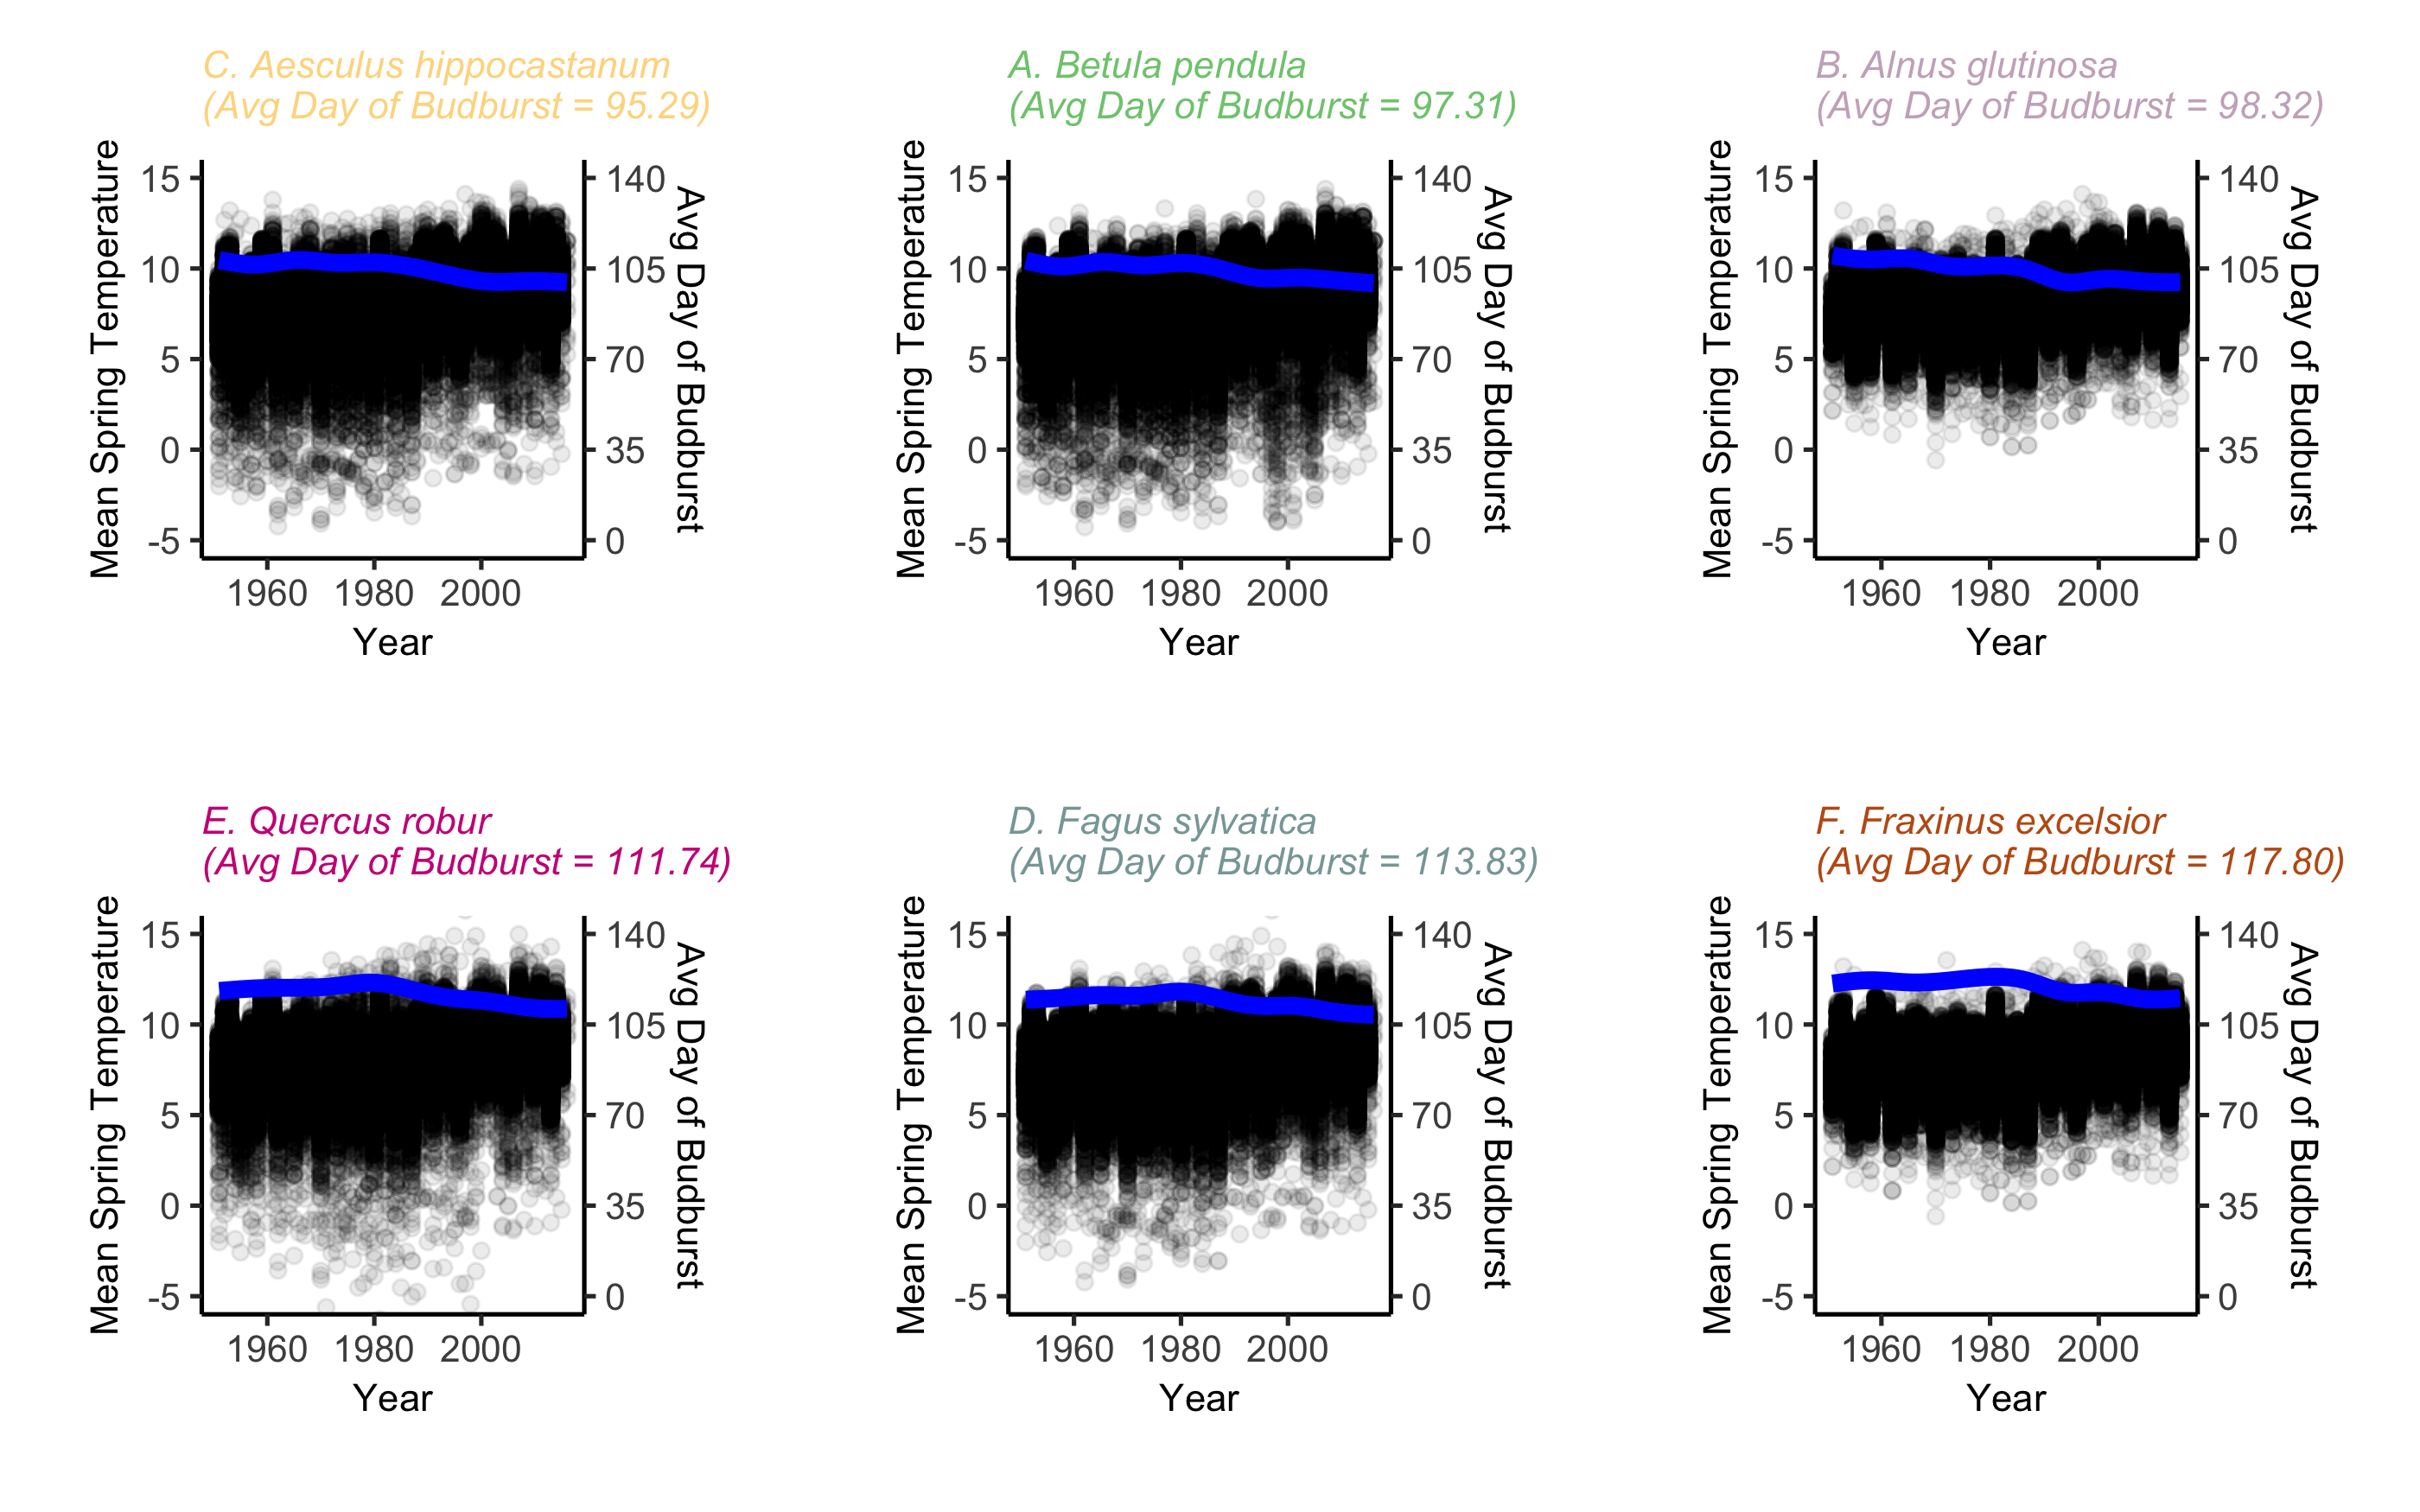
\includegraphics[width=16cm]{..//figures/MSTBB_bySpp.png}
  -\caption{Mean spring temperatures are plotted for each site over time (from 1951-2016) for each species. The blue line is a smoothing spline, indicating the trend of average day of budburst for each year for each species. Species are ordered by average day of budburst, with the earliest being \textit{Betula pendula} and the latest being \textit{Fraxinus excelsior}. }\label{fig:mst}
  -\end{center}
  -\end{figure}}
  
  
{\begin{figure} [H]
  -\begin{center}
  -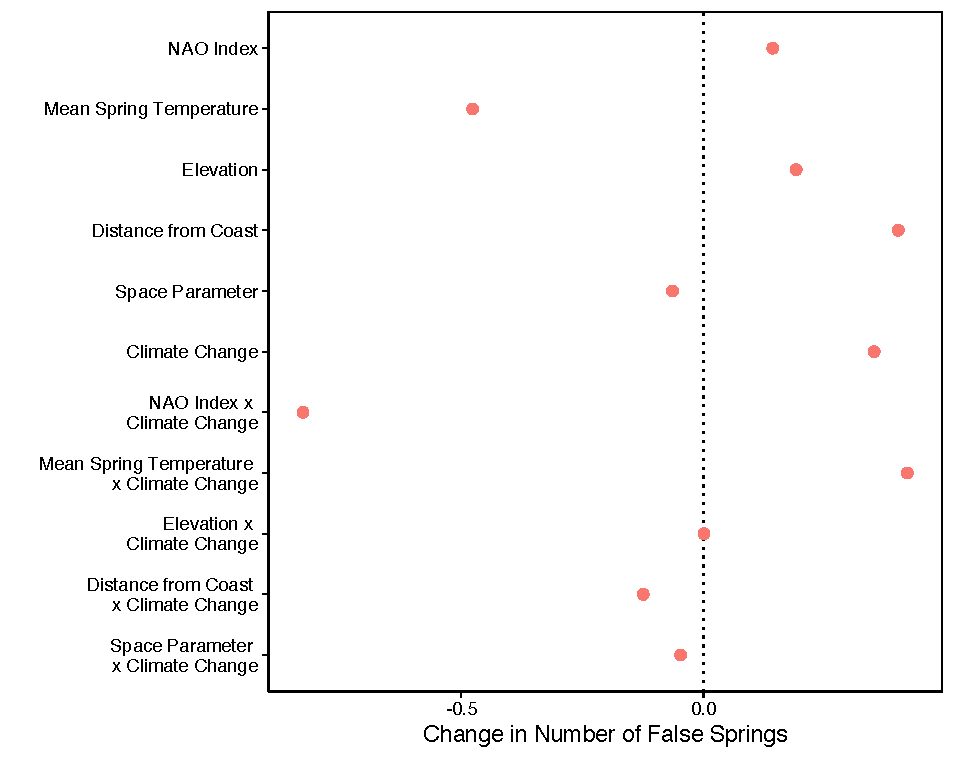
\includegraphics[width=12cm]{..//figures/model_output_orig_50.pdf}
  -\caption{Model output with standardized durations of vegetative risk for each species. More positive parameter effects indicate an increased probability of a false spring whereas more negative effects suggest a lower probability of a false spring. Uncertainly intervals are at 50\%. Parameter effects closer to zero have less of an effect on false springs. There were 743,086 zeros and 11,700 ones for false spring in the data.}\label{fig:maineffects}
  -\end{center}
  -\end{figure}}
  

{\begin{figure} [H]
  -\begin{center}
  -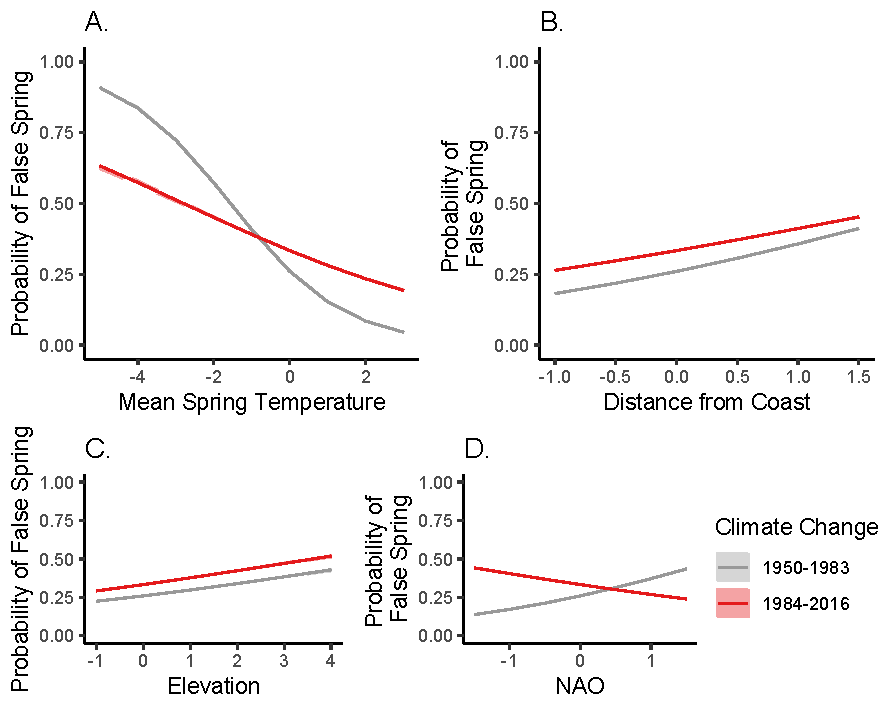
\includegraphics[width=16cm]{..//figures/InteractionPlots/IntrxnPlots_orig.pdf}
  -\caption{Plots showing the interaction effects on false spring risk for each predictor coupled with climate change. (A.) As mean spring temperature increases, there were fewer false springs but there were fewer false springs after 1983 at sites with lower mean spring temperatures. (B.) As elevation increased, false spring risk increased but there were fewer false springs at higher altitudes after 1983. (C.) As NAO indices increased, there were more false springs before 1983 but fewer after 1983. (D.) There were more false springs further from the coast and the rate of increase was consistent, however, there were fewer false springs in total after 1983. Note, the y-axis for panels A and B are from 0.00 to 1.00 but the y-axis is only from 0.00 to 0.20 for panels C and D to better see the relationships. Since we found the z-score for each predictor, the x-axis for each panel does not reflect the raw data.}\label{fig:intrxns}
  -\end{center}
  -\end{figure}}
  
{\begin{figure} [H]
  -\begin{center}
  -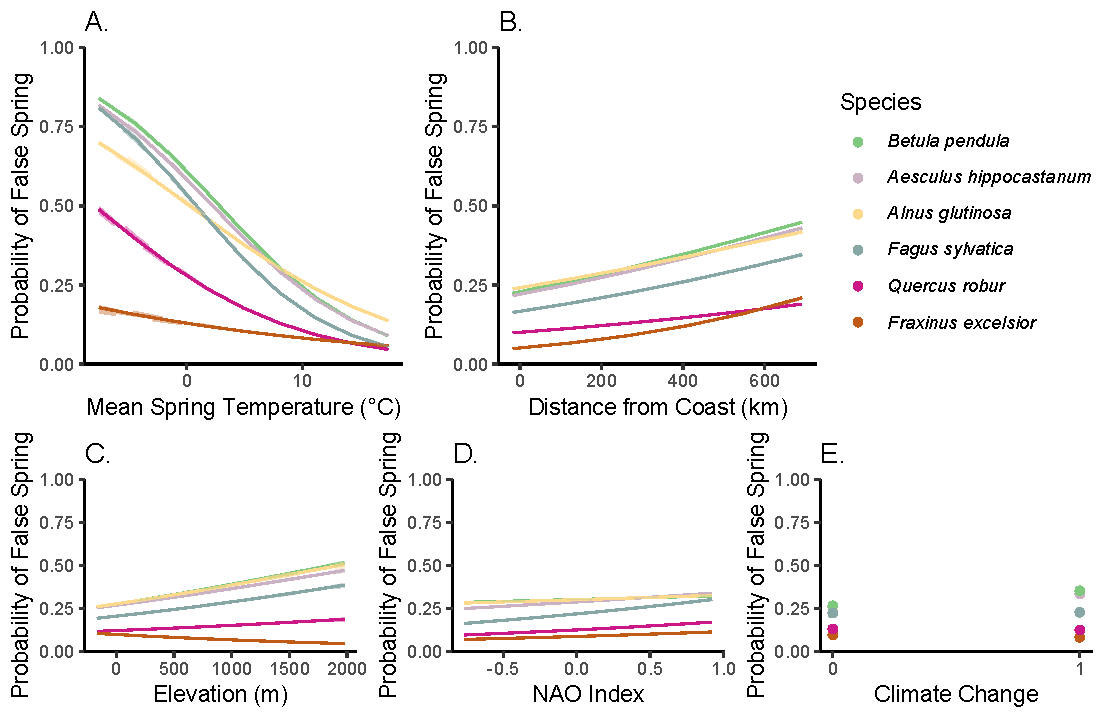
\includegraphics[width=16cm]{..//figures/InteractionPlots/Species_orig.pdf}
  -\caption{Plots showing the interaction effects of each predictor with species. (A.) As mean spring temperature increases, the probability of a false spring decreases for each species but \textit{Fraxinus excelsior} always has the lowest risk of false spring. (B.) The risk of a false spring increases with increasing altitude but the relationship is strongest for \textit{Aesculus hippocastanum} and \textit{Betula pendula}. (C.) There are slightly fewer false springs for \textit{Aesculus hippocastanum} and \textit{Betula pendula} in years with higher NAO indices. (D.) There's an increase in false spring risk for individuals further from the coast, especially for \textit{Fraxinus excelsior}. (E.) There are fewer false springs after 1983, especially for \textit{Aesculus hippocastanum} and \textit{Betula pendula}. Note, the y-axis for panels A and B are from 0.00 to 1.00 but the y-axis is only from 0.00 to 0.10 for panels C, D and E to better see the relationships. Since we found the z-score for each predictor, the x-axis for each panel does not reflect the raw data.}\label{fig:spp}
  -\end{center}
  -\end{figure}}

  



\end{document}
